\documentclass[Rapport/Playerside/GameController/GameController.tex]{subfiles}
\label{sec:playerside_gamecotroller_design}
\begin{document}
\subsubsection{Design}
I dette afsnit beskrives design for GameController klassen på playerside. Denne klasse er controller klassen for playerside, og indeholder alt den logik, der skal til, for at de 3 boundary klasser RPI\_IF, CupSensor\_IF og CupLight\_IF fungerer i et samlet system. Under designet af denne klasse har det været vigtigt at følge sekvensdiagrammet og statediagram i arkitekturet og bruge de funktioner, der har været defineret i de forskellige boundaryklasser. En del af designet af klassen bestod i også alt lave stubs for funktionerne i de 3 boundaryklasser, så det eneste der skulle gøres i en videre integrering var at slette implementeringen af stubs og bruge de rigtige funktioner. Logikken i klassen skal sørge for, at kopholder lys bliver kontrolleret korrekt. Her er de fem states i systemet vigtige, da de afgør hvordan GameController klassen skal håndterer opdateringer på kop status(CupStatus variabel) og hit status(HitStatus variabel), der ændres med metoderne updateCupStatus og updateHitStatus, som CupSensor bruger i GameController klassen. I state STARTING og PLAYING kan kop status ændres, hvorimod Hit status kun kan ændres i state PLAYING. Systemets state ændres med funktionen setState, der bruges i RPI\_IF klassen. Denne funktion håndterer de ændringer der sker lige efter en state ændringer fx så vil der ved state ændring til WON kaldes metoden ControlAllLights i CupLight klassen. Der er også en Controller metode. Dens funktion er at holde styr på ændringer i systemet. Ved en ændring af kop status vil en CupLight\_IF metoden ControlLights kaldes, når systemet er i state STARTING eller PLAYING. Om lyset blinker bliver også styret her, hvor en timer kan startes og stoppes. Ved interrupt af timeren vil funktionen Interrupt\_LED kaldes, der kontrollerer blink funktionen for de 6 kop holdere. Timeren brugt findes i PSoC creators komponent katalog og kan ses i figur \ref{fig:Timer}
\begin{figure}
    \centering 
    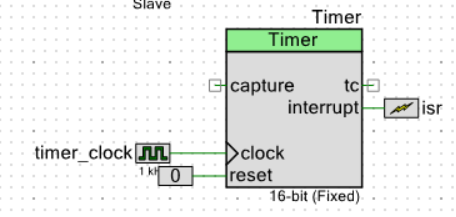
\includegraphics[width=0.5\linewidth]{Softwaredesign/GameController/graphic/gamecontroller_timer.PNG}
    \caption{Timer brugt til implementering af blink funktion}
    \label{fig:Timer}
\end{figure}
\end{document}
